\documentclass{article}
\usepackage{enumerate}
\usepackage{amsmath}
\usepackage{amssymb}
\usepackage{graphicx}
\usepackage{subfigure}
\usepackage{geometry}
\usepackage{caption}
\usepackage{indentfirst}
\usepackage{tikz}
\usetikzlibrary{circuits.logic.US}
\usetikzlibrary{arrows.meta}
\usetikzlibrary{calc}
\geometry{left=3.0cm,right=3.0cm,top=3.0cm,bottom=4.0cm}
\renewcommand{\thesection}{Problem \arabic{section}.}
\title{VE270 Homework 2}
\author{Liu Yihao 515370910207}
\date{}

\begin{document}
\maketitle

\section{}
\begin{center}
\begin{tabular}{cc|ccc}
x&y&$\rm x\oplus y'$&$\rm x'\oplus y$&$\rm(x \oplus y)'$\\
\hline
0&0&1&1&1\\
0&1&0&0&0\\
1&0&0&0&0\\
1&1&1&1&1\\
\end{tabular}
\end{center}
$$\rm x\oplus y'=x'\oplus y=(x\oplus y)'$$

\section{}
\begin{enumerate}[(a)]
\item $$\rm S\oplus E$$
\item $$\rm S+H'$$
\item $$\rm S\oplus EH'$$
\end{enumerate}

\section{}
\begin{align*}
\rm F&=\rm a'b(c+d')+a(b'+c)+a(b+d)c\\
&=\rm a'bc+a'bd'+ab'+ac+abc+acd\\
&=\rm a'bc+a'bd'+ab'+ac(1+b+d)\\
&=\rm a'bc+a'bd'+ab'+ac
\end{align*}

\section{}
\begin{align*}
\rm F'&=\rm (abc+a'b)'\\
&=\rm (abc)'(a'b)'\\
&=\rm (a'+b'+c')(a+b')\\
&=\rm aa'+ab'+ac'+a'b'+b'+b'c'\\
&=\rm 0+b'(1+a+c')+ac'\\
&=\rm b'+ac'
\end{align*}

\section{}
\begin{align*}
\rm F&=\rm a'b'c'+a'bc'+ab'c'+ab'c+abc'\\
&=\rm a'c'(b+b')+ac'(b+b')+ab'c\\
&=\rm a'c'+ac'+ab'c\\
&=\rm c'+ab'c
\end{align*}

\section{}
\begin{align*}
\rm F(a,b,b)&=\rm abc+ab+a+b+c\\
&=\rm m_1+m_2+m_3+m_4+m_5+m_6+m_7\\
&=\rm \sum m(1,2,3,4,5,6,7)
\end{align*}

\section{}
\begin{center}
	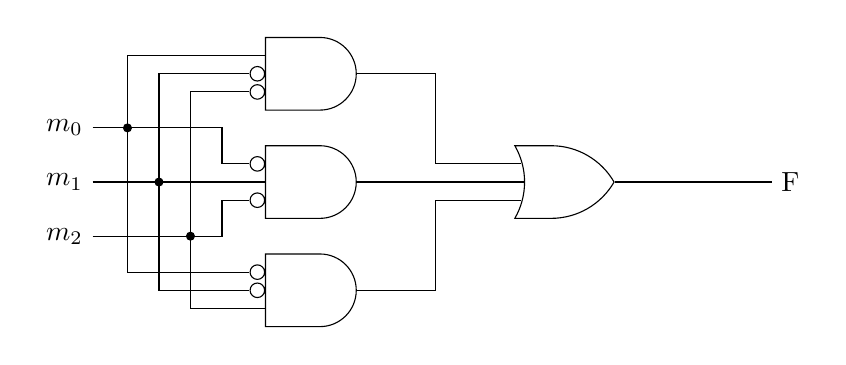
\begin{tikzpicture}[circuit logic US]
	\matrix[column sep=20mm]{
		& \node [and gate,inputs=nii,scale=1.5] (g1) {};\\
		\node (m0) {$m_0$}; \\
		\\
		\node (m1) {$m_1$}; & \node [and gate,inputs=ini,scale=1.5] (g2) {}; & \node [or gate,inputs=nnn,scale=1.5] (g4) {}; & \node (F) {F};\\
		\\
		\node (m2) {$m_2$}; \\
		& \node [and gate,inputs=iin,scale=1.5] (g3) {}; \\
	};
	\filldraw (m0)+(right:8mm) circle [radius=0.5mm];
	\filldraw (m1)+(right:12mm) circle [radius=0.5mm];
	\filldraw (m2)+(right:16mm) circle [radius=0.5mm];
	\draw (m0) -- ++(right:8mm) |- (g1.input 1) (m0) -- ++(right:20mm) |- (g2.input 1) (m0) -- ++(right:8mm) |- (g3.input 1);
	\draw (m1) -- ++(right:12mm) |- (g1.input 2) (m1) -- ++(right:12mm) |- (g2.input 2) (m1) -- ++(right:12mm) |- (g3.input 2);
	\draw (m2) -- ++(right:16mm) |- (g1.input 3) (m2) -- ++(right:20mm) |- (g2.input 3) (m2) -- ++(right:16mm) |- (g3.input 3);
	\draw (g1.output) -- ++(right:10mm) |- (g4.input 1) (g2.output) -- ++(right:10mm) |- (g4.input 2) (g3.output) -- ++(right:10mm) |- (g4.input 3);
	\draw (g4.output) -- (F);
	\end{tikzpicture}
\end{center}

\section{}
\begin{enumerate}[(a)]
\item
\begin{align*}
\rm F(a,b,b)&=\rm ab'c+abc+a'bc+abc'\\
&=\rm ab(c+c')+ac(b+b')+bc(a+a')\\
&=\rm ab+ac+bc
\end{align*}
\item \ 
\begin{center}
	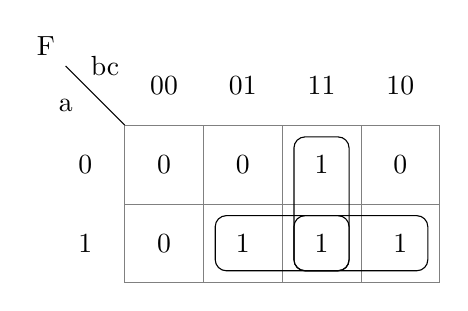
\begin{tikzpicture}
	\draw[help lines] (-2,0) grid (2,2);
\draw (-2,2) -- (-2.75,2.75);
\draw (-3,3) node {F};
\draw (-2.5,1.5) node {0} (-2.5,0.5) node {1};
\draw (-1.5,2.5) node {00} (-0.5,2.5) node {01};
\draw (0.5,2.5) node {11} (1.5,2.5) node {10};
	\draw (-2.25,2.75) node {bc} (-2.75,2.25) node {a};
	\draw (-1.5,1.5) node {0} (-0.5,1.5) node {0};
	\draw (-1.5,0.5) node {0} (-0.5,0.5) node {1};
	\draw (0.5,1.5) node {1} (1.5,1.5) node {0};
	\draw (0.5,0.5) node {1} (1.5,0.5) node {1};
	\draw (0,0.5) node[draw,rounded corners,minimum width=1.7cm,minimum height=0.7cm] {};
	\draw (1,0.5) node[draw,rounded corners,minimum width=1.7cm,minimum height=0.7cm] {};
	\draw (0.5,1) node[draw,rounded corners,minimum width=0.7cm,minimum height=1.7cm] {};
	\end{tikzpicture}
\end{center}
$$\rm F(a,b,b)=ab+ac+bc$$
\end{enumerate}

\section{}
\begin{center}
	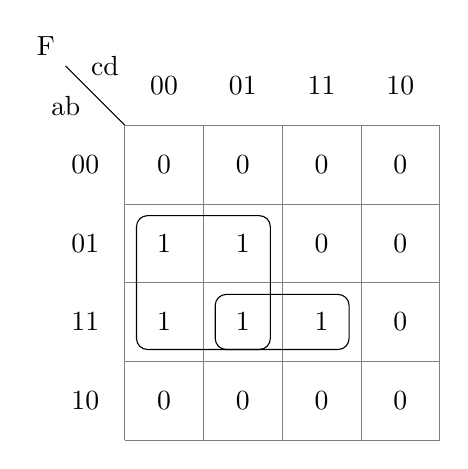
\begin{tikzpicture}
	\draw[help lines] (-2,-2) grid (2,2);
\draw (-2,2) -- (-2.75,2.75);
\draw (-3,3) node {F};
\draw (-2.5,1.5) node {00} (-2.5,0.5) node {01};
\draw (-2.5,-0.5) node {11} (-2.5,-1.5) node {10};
\draw (-1.5,2.5) node {00} (-0.5,2.5) node {01};
\draw (0.5,2.5) node {11} (1.5,2.5) node {10};
	\draw (-2.25,2.75) node {cd} (-2.75,2.25) node {ab};
	\draw (-1.5,1.5) node {0} (-0.5,1.5) node {0};
	\draw (-1.5,0.5) node {1} (-0.5,0.5) node {1};
	\draw (0.5,1.5) node {0} (1.5,1.5) node {0};
	\draw (0.5,0.5) node {0} (1.5,0.5) node {0};
	\draw (-1.5,-0.5) node {1} (-0.5,-0.5) node {1};
	\draw (-1.5,-1.5) node {0} (-0.5,-1.5) node {0};
	\draw (0.5,-0.5) node {1} (1.5,-0.5) node {0};
	\draw (0.5,-1.5) node {0} (1.5,-1.5) node {0};
	\draw (-1,0) node[draw,rounded corners,minimum width=1.7cm,minimum height=1.7cm] {};
	\draw (0,-0.5) node[draw,rounded corners,minimum width=1.7cm,minimum height=0.7cm] {};
	\end{tikzpicture}
\end{center}
$$\rm F(a,b,b)=c'd+abd$$

\section{}
\begin{center}
	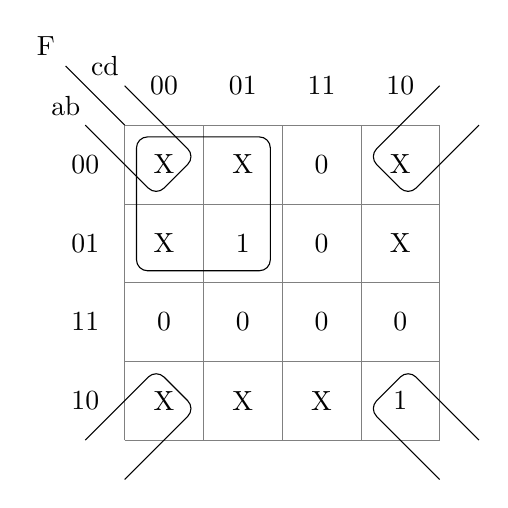
\begin{tikzpicture}
	\draw[help lines] (-2,-2) grid (2,2);
\draw (-2,2) -- (-2.75,2.75);
\draw (-3,3) node {F};
\draw (-2.5,1.5) node {00} (-2.5,0.5) node {01};
\draw (-2.5,-0.5) node {11} (-2.5,-1.5) node {10};
\draw (-1.5,2.5) node {00} (-0.5,2.5) node {01};
\draw (0.5,2.5) node {11} (1.5,2.5) node {10};
	\draw (-2.25,2.75) node {cd} (-2.75,2.25) node {ab};
	\draw (-1.5,1.5) node {X} (-0.5,1.5) node {X};
	\draw (-1.5,0.5) node {X} (-0.5,0.5) node {1};
	\draw (0.5,1.5) node {0} (1.5,1.5) node {X};
	\draw (0.5,0.5) node {0} (1.5,0.5) node {X};
	\draw (-1.5,-0.5) node {0} (-0.5,-0.5) node {0};
	\draw (-1.5,-1.5) node {X} (-0.5,-1.5) node {X};
	\draw (0.5,-0.5) node {0} (1.5,-0.5) node {0};
	\draw (0.5,-1.5) node {X} (1.5,-1.5) node {1};
	\draw (-1,1) node[draw,rounded corners,minimum width=1.7cm,minimum height=1.7cm] {};
	\draw[rounded corners] (2,2.5) -- (1.1,1.6) -- (1.6,1.1) -- (2.5,2);
	\draw[rounded corners] (-2,2.5) -- (-1.1,1.6) -- (-1.6,1.1) -- (-2.5,2);
	\draw[rounded corners] (2,-2.5) -- (1.1,-1.6) -- (1.6,-1.1) -- (2.5,-2);
	\draw[rounded corners] (-2,-2.5) -- (-1.1,-1.6) -- (-1.6,-1.1) -- (-2.5,-2);
	\end{tikzpicture}
\end{center}
$$\rm F(a,b,b)=a'c'+b'd'$$

\section{}
\begin{center}
	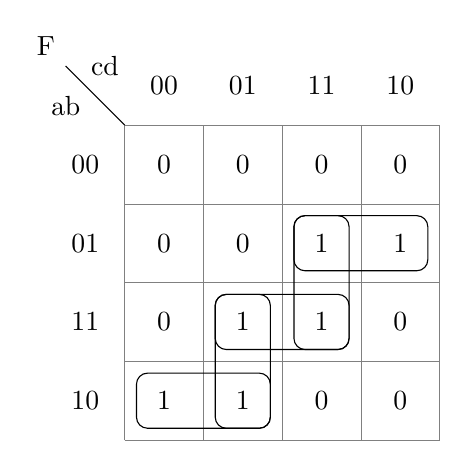
\begin{tikzpicture}
	\draw[help lines] (-2,-2) grid (2,2);
\draw (-2,2) -- (-2.75,2.75);
\draw (-3,3) node {F};
\draw (-2.5,1.5) node {00} (-2.5,0.5) node {01};
\draw (-2.5,-0.5) node {11} (-2.5,-1.5) node {10};
\draw (-1.5,2.5) node {00} (-0.5,2.5) node {01};
\draw (0.5,2.5) node {11} (1.5,2.5) node {10};
	\draw (-2.25,2.75) node {cd} (-2.75,2.25) node {ab};
	\draw (-1.5,1.5) node {0} (-0.5,1.5) node {0};
	\draw (-1.5,0.5) node {0} (-0.5,0.5) node {0};
	\draw (0.5,1.5) node {0} (1.5,1.5) node {0};
	\draw (0.5,0.5) node {1} (1.5,0.5) node {1};
	\draw (-1.5,-0.5) node {0} (-0.5,-0.5) node {1};
	\draw (-1.5,-1.5) node {1} (-0.5,-1.5) node {1};
	\draw (0.5,-0.5) node {1} (1.5,-0.5) node {0};
	\draw (0.5,-1.5) node {0} (1.5,-1.5) node {0};
	\draw (-1,-1.5) node[draw,rounded corners,minimum width=1.7cm,minimum height=0.7cm] {};
	\draw (0,-0.5) node[draw,rounded corners,minimum width=1.7cm,minimum height=0.7cm] {};
	\draw (1,0.5) node[draw,rounded corners,minimum width=1.7cm,minimum height=0.7cm] {};
	\draw (-0.5,-1) node[draw,rounded corners,minimum width=0.7cm,minimum height=1.7cm] {};
	\draw (0.5,0) node[draw,rounded corners,minimum width=0.7cm,minimum height=1.7cm] {};
	\end{tikzpicture}
\end{center}

The squared implicants are all prime implicants, but none of them is essential prime implicants.

\newpage
\section{}

\begin{center}
	original
	
	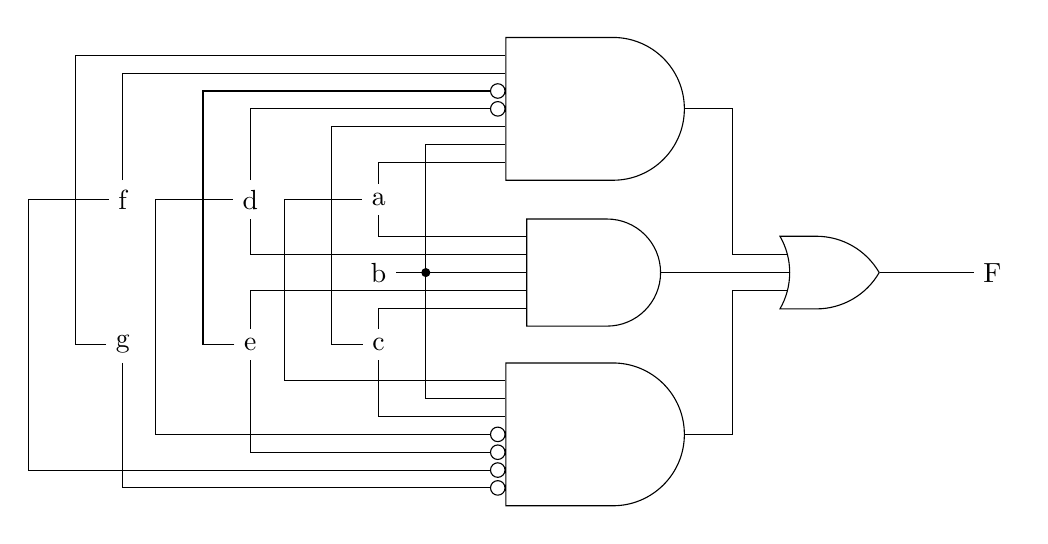
\begin{tikzpicture}[circuit logic US]
	\matrix[column sep=12mm]{
		& & & \node [and gate,inputs=nniinnn,scale=1.5] (g2) {}; \\
		\node (f) {f}; & \node (d) {d}; & \node (a) {a}; \\
		& & \node (b) {b}; & \node [and gate,inputs=nnnnn,scale=1.5] (g1) {};   & \node [or gate,inputs=nnn,scale=1.5] (g4) {}; & \node (F) {F};  \\
		\node (g) {g}; & \node (e) {e}; & \node (c) {c}; \\
		& & & \node [and gate,inputs=nnniiii,scale=1.5] (g3) {}; \\
	};
	\draw (a) |- (g1.input 1) (b) -- (g1.input 3) (c) |- (g1.input 5) (d) |- (g1.input 2) (e) |- (g1.input 4);
	\draw (a) |- (g2.input 7) (b) -- ++(right:6mm) |- (g2.input 6) (c) -- ++(left:6mm) |- (g2.input 5); 
	\draw (a) -- ++(left:12mm) |- (g3.input 1) (b) -- ++(right:6mm) |- (g3.input 2) (c) |- (g3.input 3);
	\draw (d) |- (g2.input 4) (e) -- ++(left:6mm) |- (g2.input 3) (f)  |- (g2.input 2) (g) -- ++(left:6mm) |- (g2.input 1);
	\draw (d) -- ++(left:12mm) |- (g3.input 4) (e) |- (g3.input 5) (f) -- ++(left:12mm) |- (g3.input 6) (g)  |- (g3.input 7);
	\filldraw (b)+(right:6mm) circle [radius=0.5mm];
	\draw (g1.output) -- (g4.input 2) (g2.output) -- ++(right:6mm) |- (g4.input 1) (g3.output) -- ++(right:6mm) |- (g4.input 3) (g4.output) -- (F);
	\end{tikzpicture}
	
	delay: 2 \quad gate inputs: 22
	
	\begin{align*}
	\rm F(a,b,b,d,e,f,g)&=\rm abcde+abcd'e'fg+abcd'e'f'g'\\
	&=\rm abc[de+d'e'(fg+f'g')]
	\end{align*}	
	
	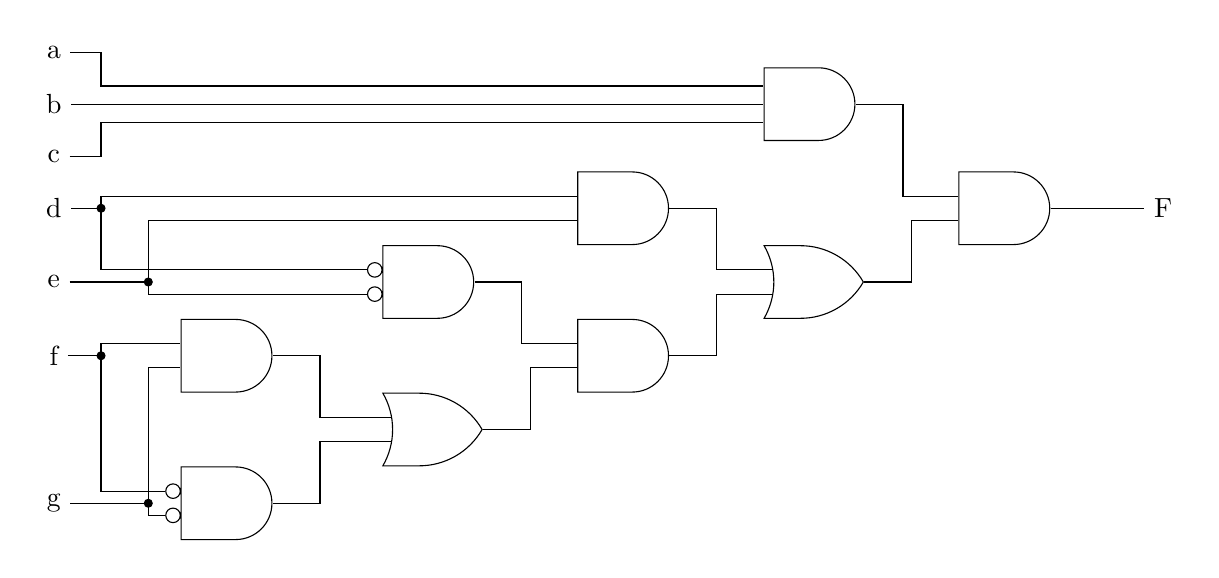
\begin{tikzpicture}[circuit logic US]
	\matrix[column sep=12mm]{
		\node (a) {a}; \\
		\node (b) {b}; & & & & \node [and gate,inputs=nnn,scale=1.5] (g1) {};\\
		\node (c) {c}; \\
		\node (d) {d}; & & & \node [and gate,scale=1.5] (g6) {}; & & \node [and gate,scale=1.5] (g10) {}; & \node (F) {F}; \\
		\node (e) {e}; & & \node [and gate,inputs=ii,scale=1.5] (g7) {}; & & \node [or gate,scale=1.5] (g9) {};\\
		\node (f) {f}; & \node [and gate,scale=1.5] (g3) {}; & & \node [and gate,scale=1.5] (g8) {}; \\
		& & \node [or gate,scale=1.5] (g5) {};\\
		\node (g) {g}; & \node [and gate,inputs=ii,scale=1.5] (g4) {};\\
	};
	\draw (a) -- ++(right:6mm) |- (g1.input 1) (b) -- ++(right:6mm) |- (g1.input 2) (c) -- ++(right:6mm) |- (g1.input 3);
	\draw (f) -- ++(right:6mm) |- (g3.input 1) (g) -- ++(right:12mm) |- (g3.input 2) (f) -- ++(right:6mm) |- (g4.input 1) (g) -- ++(right:12mm) |- (g4.input 2);
	\draw (g3.output) -- ++(right:6mm) |- (g5.input 1) (g4.output) -- ++(right:6mm) |- (g5.input 2);
	\draw (d) --++(right:6mm) |- (g6.input 1) (e) --++(right:12mm) |- (g6.input 2) (d) --++(right:6mm) |- (g7.input 1) (e) --++(right:12mm) |- (g7.input 2);
	\draw (g7.output) -- ++(right:6mm) |- (g8.input 1) (g5.output) -- ++(right:6mm) |- (g8.input 2);
	\draw (g6.output) -- ++(right:6mm) |- (g9.input 1) (g8.output) -- ++(right:6mm) |- (g9.input 2);
	\draw (g1.output) -- ++(right:6mm) |- (g10.input 1) (g9.output) -- ++(right:6mm) |- (g10.input 2) (g10.output) -- (F);
	\filldraw (d)+(right:6mm) circle [radius=0.5mm];
	\filldraw (e)+(right:12mm) circle [radius=0.5mm];
	\filldraw (f)+(right:6mm) circle [radius=0.5mm];
	\filldraw (g)+(right:12mm) circle [radius=0.5mm];
	\end{tikzpicture}
	
	delay: 5 \quad gate inputs: 19
\end{center}



\end{document}
